\documentclass[answers]{exam}
\usepackage{../preamble}
\usepackage{tikz}

\title{Graph Theory -- Sheet 2}
\author{YOUR NAME HERE :)}
\date{Trinity Term 2025}


\begin{document}
\maketitle
\begin{questions}

\question%1
For positive integers $m$ and $n$, let $K_{m, n}$ be the bipartite graph with parts $A$ and $B$ having $m$ and $n$ vertices respectively, and where every vertex of $A$ is joined to every vertex of $B$. For which $m$ and $n$ is $K_{m, n}$ Hamiltonian?



\question%2
Let $G$ be a connected graph on $n \geqslant 3$ vertices. Suppose that for every pair of non-adjacent vertices $x$ and $y$, $d(x)+d(y) \geqslant n$. Show how to find a Hamiltonian cycle in $G$ efficiently.



\question%3
Let $G$ be a connected graph with minimum degree $k$. Show that $G$ contains a path of length $\min\{n-1,2k\}$.



\question%4
Apply Dijkstra's algorithm to the graph below to find an $\ell$-shortest $v_{3} v_{4}$ path. The $\ell$ value for each edge appears alongside it.
\begin{center}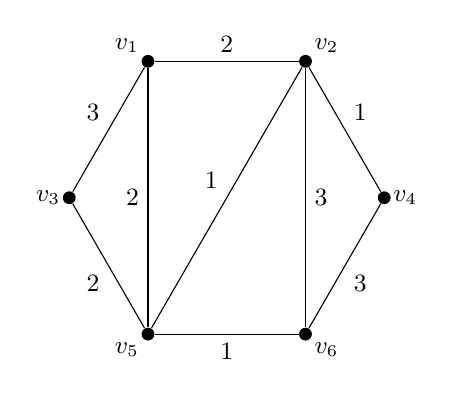
\begin{tikzpicture}
	\begin{scope}[node font=\small]
		\begin{scope}[every node/.style={circle,fill=black,inner sep=0pt,minimum size=.5em}]
			\node (1) at (120:2cm) {};
			\node (2) at (60:2cm) {};
			\node (3) at (180:2cm) {};
			\node (4) at (0:2cm) {};
			\node (5) at (-120:2cm) {};
			\node (6) at (-60:2cm) {};
		\end{scope}
		
		\node[above left] at (1) {$v_1$};
		\node[above right] at (2) {$v_2$};
		\node[left] at (3) {$v_3$};
		\node[right] at (4) {$v_4$};
		\node[below left] at (5) {$v_5$};
		\node[below right] at (6) {$v_6$};
	
		\path (1) edge node[above] {2} (2);
		\path (1) edge node[above left] {3} (3);
		\path (1) edge node[left] {2} (5);
		\path (2) edge node[above right] {1} (4);
		\path (2) edge node[above left] {1} (5);
		\path (2) edge node[right] {3} (6);
		\path (3) edge node[below left] {2} (5);
		\path (4) edge node[below right] {3} (6);
		\path (5) edge node[below] {1} (6);
	\end{scope}
\end{tikzpicture}\end{center}
Carefully describe the steps of the algorithm and the tentative distance $D$-values until they are finalized. Except for $v_{3}$, state the parent of every vertex. Finally, describe an $\ell$-shortest path tree rooted at $v_{3}$.



\question%5
Show that a graph is bipartite if and only if it does not have a cycle of odd length.



\question%6
Show that any graph has a bipartite subgraph containing at least half of its edges.



\question%7
Let $G$ be a bipartite graph in which all vertices have the same nonzero degree. Show that $G$ has a perfect matching.



\question%8
Let $G$ be a graph in which the degree of every vertex is in $\{1, \ldots, k\}$. Show that $G$ has a matching with at least $\abs{V(G)} / 2 k$ edges.



\question%9
Let $M$ be a square matrix. We say that $M$ is doubly stochastic if it has non-negative entries, every row sum is 1 and every column sum is 1. We say that $M$ is a permutation matrix if every row or column has one entry equal to 1 and all other entries equal to 0. Show that any doubly stochastic matrix $M$ can be written as $M=\sum_{i=1}^{k} c_{i} P_{i}$ for some $k$, where $P_{i}$ is a permutation matrix and $c_{i}>0$ for $1 \leqslant i \leqslant k$.

\end{questions}

\end{document}
